%!TEX program = lualatex
\documentclass[border=0mm,11pt]{standalone}
%\usepackage{color}
%\usepackage{tikz}
\usepackage[T1]{fontenc}
\usepackage[sc]{mathpazo}
\usepackage{tikz-feynman}
\usetikzlibrary {patterns,patterns.meta}
\tikzfeynmanset{compat=1.1.0}


\begin{document}

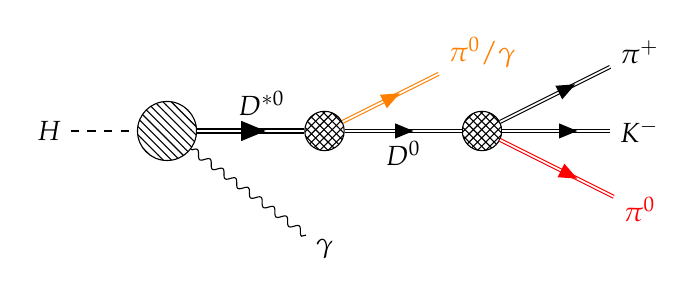
\begin{tikzpicture}[]
    \begin{feynman}
    \vertex (h) {$H$};
    \vertex [blob, right=of h, xshift=0.0cm, yshift=-0.0cm] (cent) {};
    \vertex [blob, minimum size=0.5cm, pattern=crosshatch] [right=of h, xshift=2.0cm, yshift=0.0cm] (b) {};
    \vertex [right=of h, xshift=2.0cm, yshift=-1.5cm] (f) {$\gamma$};
    \vertex [blob, minimum size=0.5cm, pattern=crosshatch] [right=of h, xshift=4.0cm, yshift=0.0cm] (p02) {};
    \vertex [right=of h, xshift=4.0cm, yshift=1.0cm, orange] (p01) {$\pi^{0}/\gamma$};
    \vertex [right=of h, xshift=6.0cm, yshift=1.0cm] (p1) {$\pi^{+}$};
    \vertex [right=of h, xshift=6.0cm, yshift=0.0cm] (p2) {$K^{-}$};
    \vertex [right=of h, xshift=6.0cm, yshift=-1.0cm, red] (p3) {$\pi^{0}$};
    \vertex [right=of h, xshift=1.2cm, yshift=0.35cm] (tag) {$D^{*0}$};
    
    \diagram* {
    (h) -- [scalar] (cent),
    (cent) -- [double, double distance=0.2ex, thick, with arrow=0.50, arrow size=0.2em] (b),
    (cent) -- [photon] (f),
    (b) -- [double, double distance=0.15ex, with arrow=0.50, arrow size=0.15em, edge label'=\(D^{0}\)] (p02),
    (b) -- [double, double distance=0.15ex, with arrow=0.50, arrow size=0.15em, orange] (p01),
    (p02) -- [double, double distance=0.15ex, with arrow=0.60, arrow size=0.15em] (p1),
    (p02) -- [double, double distance=0.15ex, with arrow=0.60, arrow size=0.15em] (p2),
    (p02) -- [double, double distance=0.15ex, with arrow=0.60, arrow size=0.15em, red] (p3),

    };
    \end{feynman}
\end{tikzpicture}

\end{document}